\documentclass[a4paper]{article}
\usepackage[top=1in,bottom=1in,left=1in,right=1in]{geometry}
\usepackage{times}
\usepackage{amssymb}
\usepackage{mathtools}	% pulls in amsmath
	\mathtoolsset{centercolon}
\usepackage{tikz}
	\usetikzlibrary{automata}
	\usepackage{tikz-qtree}
\usepackage{mathpartir}
\usepackage{amsthm}
\usepackage{amsxtra}
\usepackage{algorithm}
\usepackage{algpseudocode}
\usepackage{semantic}
	\reservestyle{\declarevars}{\texttt}
	\reservestyle{\declareops}{\texttt}
	\reservestyle{\declarestates}{\text}
\usepackage{color}
\usepackage{listings}
\usepackage{mathtools}
\usepackage[shortlabels]{enumitem}
\usepackage{graphicx}	% for pdf image
\usepackage{pgfplots}
\pgfplotsset{width=7cm}

\newtheorem{theorem}{Theorem}

\newtheorem{myexample}{\textbf{Example}}
\newtheorem{mylemma}{\textbf{Lemma}}
\newtheorem{myproof}{\textbf{Proof}}
\newtheorem{myinvariant}{\textbf{Invariant}}
\newtheorem{mytheorem}{\textbf{Theorem}}
\newtheorem{mycorollary}{\textbf{Corollary}}
\newtheorem{myapproach}{Approach}
\newtheorem{myproperty}{Property}
\newtheorem{mydefinition}{Definition}

\newtheorem{mycase}{Case}

\lstset{ %
  backgroundcolor=\color{white},   % choose the background color; you must add \usepackage{color} or \usepackage{xcolor}
  basicstyle=\small,        % the size of the fonts that are used for the code
  breakatwhitespace=false,         % sets if automatic breaks should only happen at whitespace
  breaklines=true,                 % sets automatic line breaking
  captionpos=b,                    % sets the caption-position to bottom
  commentstyle=,    % comment style
  deletekeywords={...},            % if you want to delete keywords from the given language
  escapeinside={\%*}{*)},          % if you want to add LaTeX within your code
  extendedchars=true,              % lets you use non-ASCII characters; for 8-bits encodings only, does not work with UTF-8
 % frame=single,                    % adds a frame around the code
  keepspaces=true,                 % keeps spaces in text, useful for keeping indentation of code (possibly needs columns=flexible)
  columns=fullflexible,	% not monospace
  keywordstyle=,       % keyword style
  language=Octave,                 % the language of the code
  morekeywords={forall, to, else, then, end, and, or, assign, increment, decrement, jump, jump_if, store, *, +},            % if you want to add more keywords to the set
  numbers=left,                    % where to put the line-numbers; possible values are (none, left, right)
  numbersep=5pt,                   % how far the line-numbers are from the code
  rulecolor=\color{black},         % if not set, the frame-color may be changed on line-breaks within not-black text (e.g. comments (green here))
  showspaces=false,                % show spaces everywhere adding particular underscores; it overrides 'showstringspaces'
  showstringspaces=false,          % underline spaces within strings only
  showtabs=false,                  % show tabs within strings adding particular underscores
  stepnumber=1,                    % the step between two line-numbers. If it's 1, each line will be numbered
  stringstyle=,     % string literal style
  tabsize=4,                       % sets default tabsize to 2 spaces
  title=\lstname,                  % show the filename of files included with \lstinputlisting; also try caption instead of title
  mathescape,
  belowskip=-\baselineskip,
}

\DeclareMathOperator{\prob}{prob}
\DeclareMathOperator{\dom}{dom}
\DeclareMathOperator{\rank}{rank}
\DeclareMathOperator{\key}{key}
\newcommand*{\floor}[1]{\left\lfloor{#1}\right\rfloor}
\newcommand*{\ceil}[1]{\left\lceil{#1}\right\rceil}
\newcommand{\any}{{\rule[-.2ex]{1ex}{.4pt}}}	% Less hideous than \_.
\newcommand{\RR}{\mathbb{R}}
\newcommand{\NN}{\mathbb{N}}
\newcommand{\ZZ}{\mathbb{Z}}
\newcommand{\RP}{\RR_{\ge 0}}
\newcommand*{\dave}[1]{{\color{red}\textbf{PDS: #1}}}
\newcommand{\ie}{\emph{i.e.,} }
\newcommand{\eg}{\emph{e.g.,} }
\usepackage{hyperref}
\newcommand*{\Sref}[1]{\hyperref[#1]{\S\ref*{#1}}}
\newcommand*{\figref}[1]{\hyperref[#1]{Figure~\ref*{#1}}}
\newcommand{\edge}{\longrightarrow}
\newcommand{\redge}{\longleftarrow}

\title{Exercise Sheet 9---Algorithms and Data Structures}
\author{Felipe Cerqueira \\ 2547787 \and David Swasey \\ 2542105}

\begin{document}

\maketitle

Tutorial time: Monday 14:00



\section*{Exercise 1 (10 pts)}

Some of your friends are working in a company that uses a scheduling system with a piece of old code that they can't change. When a batch of jobs arrives, the code implements the (non-sorted) greedy 2-approximation algorithm from the lecture. In the last decade since the code was written, hardware has gotten much faster, so these days computing an optimum solution for their instances seems possible. Unfortunately, the people in charge of system internals don’t allow to change the code, since it interacts with so many other parts that it’s not worth the risk of screwing up the whole system.
Your friends have come up with a workaround: Write a separate program to compute the optimal solution and then feed the jobs to the greedy algorithm in an order that will cause it to allocate them optimally. The greedy algorithm uses the machine number as tie-breaking rule in case several machines currently have the smallest load. Their question to you is this: For every instance of the load balancing problem on identical machines, is there an order of jobs such that if the greedy algorithm assigned jobs in this order, it produces an assignment with optimal makespan?
Prove the conjecture or provide a counterexample.

\paragraph{Answer.}

There is always an order such that applying the greedy algorithm leads to the optimal solution.
For example, assume that the following example is an optimal assignment $S^\ast$. 


\begin{figure}[h]
\centering
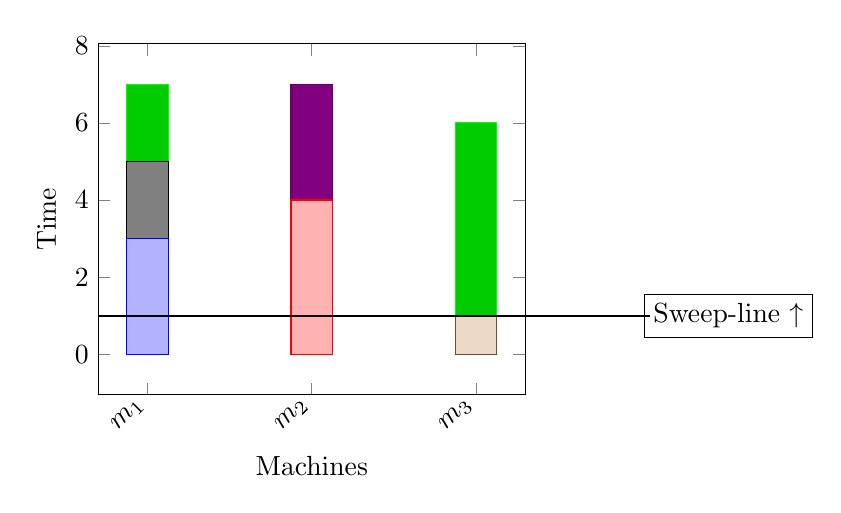
\begin{tikzpicture}
\begin{axis}[
    ybar stacked,
	bar width=15pt,
	%nodes near coords,
    enlargelimits=0.15,
    %legend style={at={(0.5,-0.20)},
    %  anchor=north},
    ylabel={Time},
    xlabel={Machines},
    symbolic x coords={$m_1$, $m_2$, $m_3$},
    xtick=data,
    x tick label style={rotate=45,anchor=east},
    ]
\addplot+[ybar] plot coordinates {($m_1$,3) ($m_2$,0) ($m_3$,0)};
\addplot+[ybar] plot coordinates {($m_1$,0) ($m_2$,4) ($m_3$,0)};
\addplot+[ybar] plot coordinates {($m_1$,0) ($m_2$,0) ($m_3$,1)};
\addplot+[ybar] plot coordinates {($m_1$,2) ($m_2$,0) ($m_3$,0)};
\addplot+[ybar] plot coordinates {($m_1$,0) ($m_2$,3) ($m_3$,0)};
\addplot+[ybar] plot coordinates {($m_1$,2) ($m_2$,0) ($m_3$,5)};
\end{axis}
\draw (0,1) -- (7,1);
\node[draw] at (8,1) {Sweep-line $\uparrow$};
\end{tikzpicture}
\end{figure}

Let's define a total order of jobs such that $j_i \prec j_k$ iff in the optimal assignment $S^\ast$, the start time of $j_i$ is earlier than the start time of $j_k$ (ties broken with machine number). We can think of this as a horizontal sweep-line going from bottom to top in the figure.

If we apply greedy in this order, every time the sweep-line intersects with the start time of a job, this job will be added to the ``most empty'' processor, producing the same allocation as the optimal assignment.


\section*{Exercise 2 (10 pts)}

The friends from the last exercise quit their jobs. They believe they are ready for the next level in their careers, and hope to get there with their start-up that manages a cloud computing system. Users of the system come with a computational task, pay for access to the system, and then have the freedom to choose any one of the m identical machines to start their task. They also have the possibility to stop their task and restart it on another machine. Users are usually impatient, and it seems they strategically pick machines to minimize completion time. Your friends have little trust in markets and wonder if it is such a good idea to give users the possibility to allocate tasks selfishly.
\begin{itemize}
	\item In an attempt to convince them, we model their system as a load balancing game on m identical machines. In the game, there are $n$ users, each user $u_j$ controls assignment of task $j$ with processing time $t_j$. In an assignment $A$ such that user $u_j$ puts task $j$ on machine $i$, the task finishes at time $c_j(A) = T_i = \sum_{k \in A(i)} t_k$. A Nash equilibrium is an assignment such that no user gets an incentive to unilaterally move its task to another machine. More formally, in Nash equilibrium $cj(A) \le t_j + \sum_{k \in A(i′)} t_k$ for all $i′ = 1,\ldots,m$. Note that in a game there might be several different assignments that represent a Nash equilibrium. Prove that every Nash equilibrium has a makespan at most twice of the optimal makespan $T \le 2T^\ast$ (that is, the price of anarchy is 2).
	\item Your friends seem to be happy about the price of anarchy, but to be fully convinced they would also like to minimize reallocation. Design a polynomial-time algorithm to compute an assignment that is a Nash equilibrium.

\end{itemize}

\paragraph{Answer.}
Attribution: We consulted notes on \emph{Selfish load balancing} by Berthold V\"ocking.

Here's a simple characterization for Nash equilibria:
\begin{equation}\label{eq:nash}
	T_{i'} \ge T_i - t_j	\qquad \text{when $j \in A(i)$}
\end{equation}

\begin{proof}[Price of anarchy]
	Let $i^\ast \in 1..m$ be a machine with highest load (if there are no machines, $T = 0$ and we're done).
	Let $j^\ast \in A(i^\ast)$ be a job with minimal cost (if there are no jobs in $A(i^\ast)$, then $T = T_{i^\ast} = 0$ and we're done).
	Assume there's at least one more job $A(i^\ast) \ni k \not= j^\ast$; otherwise $T = T_{i^\ast} = t_{j^\ast}$ so that (since every assignment must place job $j^\ast$) $T^\ast = T$ and we're done.
	By the choice of $i^\ast$, $j^\ast$, and $k$, we have $T = T_{i^\ast} \ge t_{j^\ast} + t_k \ge 2t_{j^\ast}$; that is:
	\begin{equation}\label{eq:nashij}
		t_{j^\ast} \le \frac{1}{2}T
	\end{equation}
	Thus for every $i$
	\begin{equation}\label{eq:nashi}
		T_i \underset{\eqref{eq:nash}}{\ge} T_{i^\ast} - t_{j^\ast} \underset{(i^\ast)}{=} T - t_{j^\ast} \underset{\eqref{eq:nashij}}{\ge} T - \frac{1}{2}T = \frac{1}{2}T
	\end{equation}
	To continue, we recall a bound on $T^\ast$ from lecture:
	\begin{align*}
		T^\ast &\ge \frac{1}{m} \sum_{j=1}^n t_j = \frac{1}{m} \sum_{i=1}^m T_i = \frac{1}{m} \Bigl(T_{i^\ast} + \sum_{i \not= i^\ast} T_i\Bigr) = \frac{1}{m} \Bigl(T + \sum_{i \not= i^\ast} T_i\Bigr)\\
		&\underset{\eqref{eq:nashi}}{\ge} \frac{1}{m} \bigl(T + (m-1)\frac{1}{2} T\bigr) = \frac{m+1}{2m} T
	\end{align*}
	so that $T \le \frac{2m}{m+1} T^\ast = 2T^\ast - \frac{2}{m+1}T^\ast \le 2T^\ast$.
\end{proof}

The algorithm applies the so-called \emph{max-weight best response policy}:
\begin{lstlisting}[mathescape]
	For each job $j$, sorted by decreasing $t_j$.
		$i \gets$ the least loaded machine
		$A(i) \gets A(i) \cup \{ j \}$
\end{lstlisting}
The jobs are considered in order of decreasing cost and each user makes a (locally) optimal choice when her job is considered.
The algorithm runs in time $O(n \log n)$: sort the $n$ jobs, then run $n$ iterations of the loop each taking $O(\log n)$ when using a priority queue to track machines by their current load.

\section*{Exercise 3 (10 pts)}

Consider the fractional knapsack problem where you can split items into arbitrary pieces. You should now pick $n$ numbers $x_i \in [0, 1]$ such that $\sum_i x_i w_i \le W$ and $\sum_i x_i v_i$ is maximized.
\begin{itemize}
	\item Design an algorithm to solve the fractional knapsack problem optimally in polynomial time and prove that it computes an optimal solution $x^\ast$.
	
	\paragraph{Answer.} We can use the following algorithm:
	
	\begin{enumerate}
		\item Sort the elements according to $\frac{v_i}{w_i}$ in decreasing order (best cost-benefit).
		\item Start filling the knapsack with tasks in this order until it becomes full.
	\end{enumerate}
	
	\paragraph{Proof} Assume by contradiction that $x^\ast$ is not an optimal solution. First, note that the algorithm only returns when the knapsack is full, i.e., $\sum_i x_i^\ast w_i = W$.
	
	    Since $x^\ast$ is not optimal, there exists a better solution $x'$ such that for two tasks $i\neq j$, $x_i'=x_i^\ast - \epsilon$, $x_j' = x_j^\ast + \epsilon$ and $v(x') > v(x^\ast)$. This implies that $v_j > v_i$.
	    
	    However, since the algorithm above used all tasks with largest ratio $\frac{v}{w}$, it also follows that $\frac{v_i}{w_i} > \frac{v_j}{w_j}$.
	    
	    This implies that $w_i < w_j$. However, since $\sum_i x_i^\ast w_i = W$, exchanging task $i$ for task $j$ of larger weight would overflow the knapsack's capacity. Contradiction.
	
	\medskip
	
	\item Consider the following algorithm for the non-fractional knapsack problem. Run your algorithm for the fractional problem and set $S = \{i | x_i^{\ast} = 1\}$. Show that there is no constant $c$ independent of $n$, $v$, $w$ and $W$ such that $v(S^\ast) \le c \cdot v(S)$, even when we restrict to instances with $w_i \le W$ for all items $i$ and without ties in $\frac{v_i}{w_i}$.
	
	\paragraph{Answer.}
	
	Consider each item $i$ in decreasing order (according to $\frac{v_i}{w_i}$). We can have an example where $w_1 + w_2 = W + 1$, and where for each $3 \le i \le n$, $v_i = w_i = 1$.
	Although the fractional knapsack has solution $v_1 + (1-w_1)\cdot v_2$, the modified algorithm would drop the second item and produce $v(S) = v_1$. However, the optimal solution for the non-fractional problem would be $v(S^\ast) = v_1 + (W - w_1)\cdot 1 = v_1 + W - w_1$, where we fill the knapsack with the small items.
	
	We cannot find a constant $c$ for the approximation because $\frac{v_1 + W - w_1}{v_1}$ can be made arbitrarily large if we increase $W$ while maintaining $w_1 + w_2 = W+ 1$.
	
	\medskip
	
	\item Show how to adjust the algorithm and the definition of $S$ such that the statement holds for $c=2$. Show that the analysis is tight.
	\paragraph{Answer.}

	We can do the allocation as follows:
	
		\begin{enumerate}
		\item Sort the items according to $\frac{v_i}{w_i}$ in decreasing order.
		\item Keep putting items in the knapsack, until item $k$ doesn't fit.
		\item Return $\max\{\sum\limits_{i<k} v_i, v_k\}$.
	\end{enumerate}

Let $S^G$ and $S^\ast$ be the greedy solution and the optimal solutions to the non-fractional knapsack, and let $S^f$ be the optimal solution to the fractional knapsack.

Note that $v(S^f) = \sum\limits_{i < k}{v_i} + \alpha \cdot v_k$, where $\alpha$ is the fraction of the task $k$ that does not fit.

Since the non-fractional solution can never be better than the fractional solution:

$$v(S^\ast) \le v(S^f) = \sum\limits_{i < k}{v_i} + \alpha \cdot v_k \le \sum\limits_{i<k} v_i + v_k \le 2 \max \left \{\sum\limits_{i<k} v_i, v_k \right \} \le 2 v(S^G).$$

To show the analysis is tight, consider the following example.
Capacity $W = 2x$, and the items are $(v_1 = x + 2, w_1 = x + 1)$, $(v_2=x, w_2=x), (v_3=x-1, w_3 = x)$.

The optimal algorithm returns $v_2 + v_3 = 2x-1$ with maximum weight $2x$, while the greedy algorithm returns $v_1 = x+2$ and total weight $x+1$, without being able to add more items. Thus, the approximation factor converges to $2$ for large values of $x$.

\end{itemize}



\section*{Exercise 4 (10 pts)}

Instead of matching into pairs, we here consider the 3-dimensional matching problem. We are given disjoint sets $X$, $Y$, $Z$ and a set $T \subseteq X \times Y \times Z$ of ordered triples. A subset $M \subseteq T$ is a 3-dimensional matching if each element of $X \cup Y \cup Z$ is contained in at most one triple. The goal is to find a 3-dimensional matching $M$ of maximum cardinality. Give a polynomial-time 3-approximation algorithm that finds $M$ with $|M| \le 3|M^\ast|$.

\paragraph{Answer.}

We can use a greedy algorithm to obtain a maximal 3-dimensional matching.

\begin{lstlisting}[mathescape]
	$M \gets \{t\}$, where $t$ is any triple in set $T$.
	For each triple $t'$ in $T \setminus \{t\}$:
		For each triple $t$ in $S$:
			if $t'$ intersects $t$:
				break
		$M \gets M \cup \{t'\}$
\end{lstlisting}

Let $M$ be any maximal 3-dimensional matching, and let $M^\ast$ be the maximum 3-dimensional matching.

For each triple $t = \{x,y,z\} \in M^\ast$, there can be only two cases:
\begin{enumerate}
	\item Neither of the three vertices $\{x,y,z\}$ are covered by $M$. But this case is impossible, since $M$ is maximal.
	\item At least one of the three vertices $\{x,y,z\}$ is covered by $M$.
\end{enumerate}

Since for each of three vertices in $M^\ast$, at least one is in $M$, then $|M| \le 3|M^\ast|$.

------------------------------------------------------------------------------------------

I was also wondering if we cannot compute bipartite matchings for pairs $(x,y,-)$, $(x,-,z)$ and $(-,y,z)$, and then try to intersect them to obtain the 3-dimensional matching with better approximation factor. For example, we could start by computing the maximum bipartite matching in $X \cup Y$, convert these edges into vertices and them compute a bipartite matching between these vertices and vertices in $Z$. But I don't know if this works.

\section*{Exercise 5 (10 pts)}

The pricing method for vertex cover obtains a 2-approximation. Show how to adjust it to obtain an optimal vertex cover in bipartite graphs in polynomial time by relating prices to flows and vertex covers to cuts.

\paragraph{Answer.}

\end{document}
